\documentclass[aspectratio=169]{beamer}

\usetheme{Madrid}
\usecolortheme{default}

\usepackage[utf8]{inputenc}
\usepackage[T1]{fontenc}
\usepackage{booktabs}
\usepackage{tikz}
\usetikzlibrary{arrows.meta,positioning}

\title[Election Analytics Platform]{Election Analytics Platform for Portugal}
\subtitle{Advanced Topics in Databases Practical Assignment}
\author{Rui Coelho, up202106772 \and Ricardo Ribeiro, up202104806}
\date{June 2026}

\tikzset{
  box/.style={draw, rounded corners=1mm, align=center, minimum width=2.7cm, minimum height=0.85cm, font=\small},
  arrow/.style={-{Latex[length=2mm]}, line width=0.5pt}
}

\begin{document}

\begin{frame}
  \titlepage
\end{frame}

\begin{frame}{Goal and Scope}
  \begin{itemize}
    \item Database-centred platform for analysing Portuguese election results.
    \item Datasets: official CNE Autarquicas 2013, 2017, 2021, and 2025 spreadsheet packages.
    \item Spatial layer: official DGT CAOP GeoPackages loaded into PostGIS.
    \item Thin Flask frontend using explicit SQL through \texttt{psycopg2}.
  \end{itemize}
\end{frame}

\begin{frame}{Architecture}
  \centering
  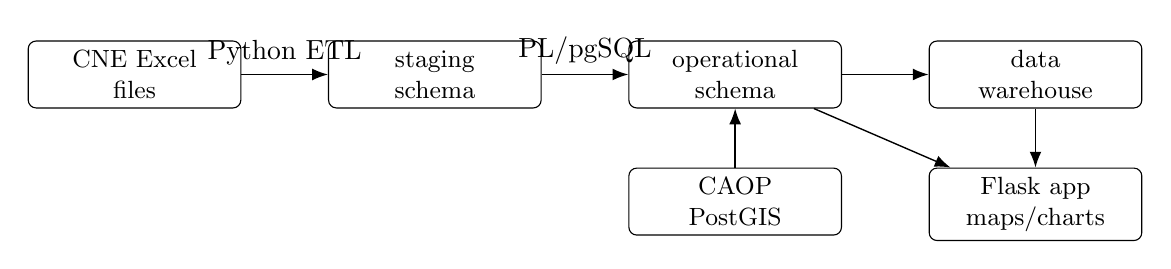
\begin{tikzpicture}[node distance=0.75cm and 1.1cm]
    \node[box] (cne) {CNE Excel\\files};
    \node[box, right=of cne] (staging) {staging\\schema};
    \node[box, right=of staging] (operational) {operational\\schema};
    \node[box, right=of operational] (warehouse) {data\\warehouse};
    \node[box, below=of operational] (caop) {CAOP\\PostGIS};
    \node[box, below=of warehouse] (app) {Flask app\\maps/charts};

    \draw[arrow] (cne) -- node[above]{Python ETL} (staging);
    \draw[arrow] (staging) -- node[above]{PL/pgSQL} (operational);
    \draw[arrow] (operational) -- (warehouse);
    \draw[arrow] (caop) -- (operational);
    \draw[arrow] (warehouse) -- (app);
    \draw[arrow] (operational) -- (app);
  \end{tikzpicture}
\end{frame}

\begin{frame}{Operational Model}
  \begin{itemize}
    \item Core entities: elections, organs, territories, candidacies.
    \item Result entities: turnout, vote results, seat results, elected members.
    \item Territory hierarchy supports district/region, municipality, and parish drill-down.
    \item Candidacies model parties, coalitions, and citizen groups through a typed local candidacy table.
    \item Keys, constraints, uniqueness rules, and indexes support integrity and dashboard queries.
  \end{itemize}
\end{frame}

\begin{frame}{ETL Pipeline}
  \begin{itemize}
    \item Rerunnable Python loader parses the CNE spreadsheets and populates staging.
    \item Loader is parameterized by source folder, election code, election name, and election date.
    \item PL/pgSQL procedure transforms staging rows into normalized operational tables.
    \item Warehouse refresh rebuilds dimensions and facts from the operational schema.
    \item CAOP loader reads GeoPackages, reprojects to EPSG:3763, and updates territory geometries.
  \end{itemize}

  \vspace{0.2cm}
  \begin{table}
    \begin{tabular}{lr}
      \toprule
      Election & Vote rows\\
      \midrule
      AL2013 & 12152\\
      AL2017 & 12069\\
      AL2021 & 12277\\
      AL2025 & 12839\\
      \bottomrule
    \end{tabular}
  \end{table}
\end{frame}

\begin{frame}{Warehouse and Analytical SQL}
  \begin{itemize}
    \item Star schema: election, organ, territory, and candidacy dimensions.
    \item Central fact table stores votes, official percentages, mandates, and turnout measures.
    \item Analytical SQL includes:
      \begin{itemize}
        \item D'Hondt mandate allocation;
        \item three window-function queries;
        \item \texttt{ROLLUP} and \texttt{CUBE};
        \item \texttt{FILTER} and JSON aggregation.
      \end{itemize}
    \item Historical SQL compares turnout, vote-share trends, winner changes, and seat changes across 2013/2017/2021/2025.
  \end{itemize}
\end{frame}

\begin{frame}{SQL Programming}
  \begin{itemize}
    \item SQL functions: vote share, turnout rate, D'Hondt allocation.
    \item PL/pgSQL procedures: load operational schema from staging; refresh warehouse.
    \item Triggers enforce meaningful business rules:
      \begin{itemize}
        \item no negative turnout/vote/mandate values;
        \item blank plus null votes cannot exceed voters;
        \item vote and seat rows must match the candidacy scope.
      \end{itemize}
  \end{itemize}
\end{frame}

\begin{frame}{Spatial and Frontend}
  \begin{itemize}
    \item PostGIS stores geometries as \texttt{geometry(MultiPolygon, 3763)}.
    \item Loaded geometry coverage:
      \begin{itemize}
        \item district/region: 20 / 20;
        \item municipality: 308 / 308;
        \item parish: 3241 / 3394 after the four-election load.
      \end{itemize}
    \item Frontend includes election/organ selection, interactive Leaflet municipality map, result table, turnout summary, vote-share chart, seat chart, and historical comparison page.
  \end{itemize}
\end{frame}

\begin{frame}{Validation}
  \begin{itemize}
    \item PostgreSQL validation checks staging, operational, warehouse, materialized views, and D'Hondt results.
    \item Four loaded elections: AL2013, AL2017, AL2021, and AL2025.
    \item Agueda municipal council D'Hondt matches official mandates:
      \begin{itemize}
        \item PPD/PSD.MPT: 4;
        \item PS: 2;
        \item CDS-PP: 1.
      \end{itemize}
    \item Flask endpoint tests:
      \begin{itemize}
        \item homepage returned HTTP 200;
        \item municipality results returned HTTP 200;
        \item map endpoint returned 308 municipality features.
      \end{itemize}
  \end{itemize}
\end{frame}

\begin{frame}{Limitations and Extensions}
  \begin{itemize}
    \item Implemented extensions: historical comparisons, parish-level support, materialized views/precomputed aggregates, interactive map drill-down, and frontend comparison views.
    \item CAOP 2025 is used instead of CAOP 2021; it is official DGT data but not a perfect historical match.
    \item Parish geometries are partial because some codes changed across election cycles.
    \item Some elected-member rows do not match normalized parish candidacies exactly.
    \item Future work: multiple election types, election-type-specific frontend views, and improved parish reconciliation.
  \end{itemize}
\end{frame}

\begin{frame}{Demo Path}
  \begin{enumerate}
    \item Show the repository structure and SQL/ETL files.
    \item Run validation query for Agueda D'Hondt.
    \item Open the historical comparison page for vote-share trends and winner changes.
    \item Open the Flask map and select a municipality.
    \item Show result table, turnout, vote-share chart, seat chart, and elected members.
  \end{enumerate}
\end{frame}

\end{document}
